\documentclass[UTF8,fontset=none,a4paper,11pt,twoside]{ctexart}

% ---------- 基础排版 ----------
\usepackage{geometry}
\geometry{left=2.5cm,right=2cm,top=2.5cm,bottom=2.5cm}
\setlength{\headheight}{14pt}
\raggedbottom
\setlength{\emergencystretch}{1em}
\setlength{\parindent}{0pt}
\setlength{\parskip}{0.6em}

% ---------- 数学、图表与代码 ----------
\usepackage{amsmath,amssymb,amsthm}
\usepackage{graphicx}
\graphicspath{{figures/}}
\usepackage{booktabs,array,tabularx}
\usepackage{enumitem}
\usepackage{placeins}
\usepackage{needspace}
\usepackage{float}
\usepackage{etoolbox}
\pretocmd{\section}{\FloatBarrier}{}{}
\ctexset{
  section = {name = {}, number = \arabic{section}, indent = 0pt, format = \raggedright\Large\bfseries},
  subsection = {indent = 0pt, format = \raggedright\large\bfseries},
  subsubsection = {indent = 0pt, format = \raggedright\large\bfseries}
}
\setcounter{tocdepth}{3}
\setcounter{secnumdepth}{3}

\usepackage{forest}
\usepackage{xcolor}
\usepackage{listings}
\setCJKmainfont{TeX Gyre Termes}[Script=Latin]
\setCJKmonofont{TeX Gyre Cursor}[Script=Latin]
\setmainfont{TeX Gyre Termes}
\setsansfont{TeX Gyre Heros}
\setmonofont{DejaVu Sans Mono}[Scale=MatchLowercase]
\newfontfamily\titlefont{TeX Gyre Termes}

\definecolor{codegreen}{RGB}{0,110,45}
\definecolor{codeblue}{RGB}{0,70,170}
\definecolor{codegray}{RGB}{100,100,100}

\lstdefinestyle{ads}{
  basicstyle=\ttfamily\small,
  numbers=left,
  numberstyle=\tiny\color{codegray},
  frame=tb,
  tabsize=4,
  columns=fullflexible,
  keepspaces=true,
  showstringspaces=false,
  commentstyle=\color{codegreen},
  keywordstyle=\color{codeblue}\bfseries,
  breaklines=true
}
\lstset{style=ads,language=C}

% ---------- Theorem环境 ----------
\newtheorem{theorem}{Theorem}[section]
\newtheorem{lemma}[theorem]{Lemma}
\newtheorem{proposition}[theorem]{Proposition}
\newtheorem{claim}[theorem]{Claim}
\newtheorem{corollary}[theorem]{Corollary}
\theoremstyle{definition}
\newtheorem{definition}[theorem]{Definition}

% ---------- 链接（尽量最后加载） ----------
\usepackage[hidelinks]{hyperref}
\usepackage{fancyhdr}
\pagestyle{fancy}
\fancyhf{}
\fancyhead[R]{\thepage}
\renewcommand{\headrulewidth}{0pt}
\fancypagestyle{plain}{%
  \fancyhf{}
  \fancyhead[R]{\thepage}
  \renewcommand{\headrulewidth}{0pt}%
}

% ---------- 只需修改这里 ----------
\newcommand{\ProjectTitle}{Compare Search Trees}
\newcommand{\StudentNames}{Author pending}
\newcommand{\GroupNumber}{Group pending}
\newcommand{\ProjectDate}{2026-10-03}
\newcommand{\ReportStatus}{Draft: cover metadata awaiting author and group}


\renewcommand{\figurename}{Figure}
\renewcommand{\tablename}{Table}
\renewcommand{\lstlistingname}{Listing}
\renewcommand{\abstractname}{Abstract}
\renewcommand{\contentsname}{Contents}
\renewcommand{\refname}{Reference}
\renewenvironment{abstract}{%
  \begin{center}
    {\bfseries\fontsize{14pt}{17pt}\selectfont Abstract\par}
  \end{center}
  \begin{quotation}\normalsize
}{%
  \end{quotation}
}

\makeatletter
\renewcommand*{\l@subsubsection}[2]{%
  \@dottedtocline{3}{3.8em}{3.2em}{#1}{#2}%
}
\makeatother
\begin{document}

\begin{center}
  \vspace*{0.3cm}
  {\titlefont\bfseries\fontsize{20pt}{25pt}\selectfont
    \ProjectTitle\par}

  \vspace{1.2cm}
  {\titlefont\bfseries\fontsize{13pt}{17pt}\selectfont
    \StudentNames\par}

  \vspace{0.25cm}
  {\titlefont\fontsize{11pt}{14pt}\selectfont
    \GroupNumber\par}

  \vspace{0.9cm}
  {\titlefont\bfseries\fontsize{12pt}{15pt}\selectfont
    Date: \ProjectDate\par}
\end{center}

\vspace{0.8cm}

\begin{center}
\textit{\ReportStatus}
\end{center}
\begin{abstract}
Five search-tree implementations are compared on three prescribed insertion/deletion sequences at seven sizes from 1,000 to 100,000 distinct integers. Correctness is checked by an insert/delete smoke test per tree, run under memory and undefined-behavior sanitizers. Each timed configuration is repeated three times, and exact inputs and raw timings are retained. Ordered BST insertion exhibits quadratic growth, while balanced and adaptive trees avoid that total-cost behavior. Phase-separated plots reveal the strong effect of deletion order and the benefits of splaying on ordered sequences. Results apply to the submitted in-memory C implementations on the measured WSL2 environment.

\end{abstract}

\clearpage
\tableofcontents
\clearpage

\section{Introduction}

\subsection{Background and Objectives}

A search tree represents an ordered set while supporting insertion, deletion, and membership queries. The same set can have very different update costs because its representation depends on balance rules and access order. This project compares an unbalanced binary search tree (BST), an AVL tree, a splay tree, a red-black tree, and a B+ tree using the three update sequences required by Project 8-1, Compare Search Trees.

Each tree is implemented in its own C file, src/\allowbreak{}bst.c, src/\allowbreak{}avl.c, src/\allowbreak{}splay.c, src/\allowbreak{}redblack.c, and src/\allowbreak{}bplus.c, written in the style of the supplied testavl.c. Each file holds one node type and its operations. The driver in src/\allowbreak{}test.c includes those five files and runs either the smoke test or the timed benchmark.

\subsection{Problem Statement}

For each size N, the keys are the N distinct integers from 0 through N-1. The experiment inserts every key into an empty tree and then deletes every key. Scenario 1 inserts in increasing order and deletes in increasing order; Scenario 2 inserts in increasing order and deletes in decreasing order; Scenario 3 uses separately shuffled insertion and deletion permutations. The measured sizes are 1,000, 2,000, 5,000, 10,000, 20,000, 50,000, and 100,000.

\section{Data Structure / Algorithm Specification}

\subsection{Interface and Representation}

\begin{table}[H]
\centering
\small
\caption{Implemented tree representations.}
\begin{tabularx}{\textwidth}{lXX}
\toprule
File & Representation & Structural invariant \\
\midrule
bst.c & Key and two child links & Strict binary-search ordering \\
avl.c & BST node plus cached height & Child heights differ by at most one \\
splay.c & Key and two child links & Ordering; accessed updates restructure the root \\
redblack.c & BST node plus a color flag & Black root; equal black heights; no adjacent reds \\
bplus.c & Arrays, cached minimum, child links, leaf Next & Half-full nonroot nodes; equal leaf depths \\
\bottomrule
\end{tabularx}
\end{table}
\FloatBarrier

Every tree exposes the same four operations. Insert(X,T) and Delete(X,T) return the updated root and callers must assign it; duplicate insertion stores no additional record, and deleting an absent key preserves the set. Find(X,T) returns Boolean membership, and MakeEmpty(T) frees the tree and returns NULL. Find is read-only everywhere; the splay module therefore does not splay on Find, and search performance is outside this comparison.

\subsection{Unbalanced Binary Search Tree}

Insertion follows comparison-selected links to a NULL child, using a pointer to the owning link so the root and lower nodes are updated uniformly. Deletion bypasses a node with at most one child and otherwise copies the inorder successor into it before unlinking the successor. All operations, including destruction, are iterative, so even a 100,000-node chain cannot overflow the recursion stack.

\subsection{AVL Tree}

An empty subtree has height -1. Each recursive update repairs the search path on return, choosing a single or double rotation from the cached child heights and refreshing them after structural changes. Using child heights rather than the inserted key is essential for deletion, including when the heavier child has equal-height children, and deletion may reduce height repeatedly, so every affected ancestor is rebalanced.

\begin{lstlisting}[language={},numbers=none]
AVL-DELETE(X,T):
    if T is empty: return empty
    descend left or right according to comparison
    on a match with two children:
        copy the minimum key of T.right
        recursively delete that successor
    on a match with at most one child:
        free T and return its remaining child
    repair balance and height; return the new root
\end{lstlisting}

\subsection{Splay Tree}

Top-down splaying uses a temporary header and two partial trees; zig-zig rotations shorten repeated-direction paths, and final assembly attaches smaller keys left of the accessed root and larger keys right. Insertion splays around X and makes the new key the root; deletion splays X and, if present, joins the remaining subtrees by splaying the maximum of the left subtree. Updates restructure the tree instead of maintaining an explicit height constraint, giving an O(log N) amortized bound per operation but O(N) worst-case cost for a single one. \href{https://www.cs.cmu.edu/~sleator/papers/Self-Adjusting.htm}{Source: Sleator and Tarjan, Self-Adjusting Binary Search Trees}.

\subsection{Red-Black Tree}

The implementation is the left-leaning red-black (LLRB) variant, which encodes a 2-3 tree through link colors: a new node is red, rotations restore left-leaning links, color flips split represented 4-nodes, and the root stays black. Deletion reddens an all-black-child root and uses MoveRedLeft or MoveRedRight before descending into a represented 2-node, replacing a two-child match by its successor and repairing the return path. Measured constants are specific to this variant. \href{https://algs4.cs.princeton.edu/code/edu/princeton/cs/algs4/RedBlackBST.java.html}{Source: Princeton, RedBlackBST implementation}.

\subsection{B+ Tree}

CAPACITY is 32 and MINIMUM is half of it, and the minimum occupancy is the value that is really constrained. A node that loses an entry falls to 15 entries, its smallest possible sibling holds 16, and 15+16=31 stays within the legal capacity of 32, so a merge never overflows and deletion never has to split. Any minimum above half the capacity would break that, which makes 16 the largest safe value for capacity 32. Capacity is a design parameter, and the minimum occupancy must be chosen consistently with it. At capacity 32, an internal routing search uses at most 5 key comparisons; the lower-bound search in a full 32-record leaf can require 6. A tree containing 100,000 records has exactly four levels, counting the root and leaves: three levels hold at most 32\textasciicircum{}3 = 32,768 records, whereas five levels require at least 2 * 16\textasciicircum{}4 = 131,072. A nonroot node holds 16 to 32 children or leaf records. An internal root holds 2 to 32 children, while a leaf root holds 1 to 32 records; an empty tree is represented by NULL. Records live only in leaves, whose Next links form a sorted chain; internal separator i is the cached minimum of child i+1, so equality routes right, and Refresh recomputes cached minima after every update. Insertion shifts the leaf suffix and propagates splits upward, an overflow of 33 splitting into 16 and 17. Deletion repairs a deficient child on the return path by borrowing from a sibling holding more than 16 entries or merging the deficient node with a minimally occupied sibling; leaf merges repair Next and a one-child root is replaced by its child. \href{https://cs186berkeley.net/notes/note4/}{Source: Berkeley CS 186, B+ Trees}.

\begin{lstlisting}[language={},numbers=none]
BPLUS-REPAIR(parent,i):
    if child[i] has at least 16 entries: return
    if left sibling has more than 16 entries:
        move its last entry to the front of child[i]
    else if right sibling has more than 16 entries:
        move its first entry to the end of child[i]
    else:
        concatenate adjacent children and remove one parent link
        repair the leaf Next link when merging leaves
    refresh child minima and parent separators
\end{lstlisting}

\subsection{Correctness Argument}

Insertion and deletion change the represented set by at most one key, and successor replacement and rotations preserve search ordering because the successor is the smallest key in the right subtree and the middle subtree stays between the rotated keys. Each repair restores its representation invariant: AVL heights, red-black black-height and color balance, splay key partitions, and B+ occupancy with separator routing. Induction over the update sequence therefore preserves set semantics and every invariant. The smoke test below exercises that argument on concrete inputs, but passing it is not a proof for all inputs.

\section{Testing Results}

\subsection{Environment and Timing Methodology}

\begin{table}[H]
\centering
\small
\caption{Measured experiment environment.}
\begin{tabularx}{\textwidth}{lX}
\toprule
Item & Configuration \\
\midrule
Experiment date & 2026-10-03 \\
CPU & AMD Ryzen 7 H 255 W/ Radeon 780M \\
Operating system & WSL2; Linux 6.6.87.2-microsoft-standard-WSL2; x86-64 \\
Compiler & gcc (Ubuntu 13.3.0-6ubuntu2\textasciitilde{}24.04.1) 13.3.0 \\
Build flags & -std=c11 -O2 -Wall -Wextra -Wpedantic \\
Timer & POSIX CLOCK\_MONOTONIC, elapsed wall time \\
Repetitions & 3 for each scenario / size / tree \\
Execution & One process; sequential; no CPU affinity \\
B+ capacity & 32 leaf records or 32 internal children \\
\bottomrule
\end{tabularx}
\end{table}
\FloatBarrier

Insertion and deletion are timed separately with CLOCK\_\allowbreak{}MONOTONIC. Allocation and freeing inside tree operations are included; input generation, file output, and membership checks are excluded. A 256-key untimed run warms each implementation, and the execution order rotates across trials. Between the timed phases, 256 read-only queries sample inserted keys; after deletion, the driver requires a NULL root. No structural invariant checker runs in the current driver. The queries may warm deletion caches.

\subsection{Smoke Test}

\begin{table}[H]
\centering
\small
\caption{Observed smoke test results.}
\begin{tabularx}{\textwidth}{XlX}
\toprule
Test case & Type & Expected / actual result \\
\midrule
Deleting from an empty tree & Boundary & Accepted, no change; PASS for all five trees \\
INT\_MIN and INT\_MAX; 1,000 increasing keys & Functional & Both boundary keys found; sampled keys found; an absent key reported absent \\
Full insert-then-delete cycle & Functional & Every key accepted, then removed; NULL root afterwards; PASS \\
Same cycle under ASan and UBSan & Memory / undefined behavior & No sanitizer diagnostics; PASS \\
All 315 timed trials, N up to 100,000 & Large-scale & Sampled keys present after insertion; NULL root after deletion; PASS \\
\bottomrule
\end{tabularx}
\end{table}
\FloatBarrier

README.md documents how to reproduce every result in this chapter: make check runs the cycle above, make sanitize repeats it under AddressSanitizer and UndefinedBehaviorSanitizer, and make benchmark regenerates all input files and timings. The checks.log file retains the compiler commands and the PASS output from both builds. Sanitizers detect exercised memory errors and undefined behavior, but do not verify AVL height balance, red-black black heights, or B+ occupancy and separator invariants. The smoke test checks sampled membership and a full deletion cycle; it does not replace those structural checks.

\subsection{Runtime Tables}

All values below are milliseconds. Each total is the median of three per-trial insertion-plus-deletion sums. The separate insertion and deletion medians are computed independently and need not add exactly to the median total. Minimum and maximum values describe the three observed runs, not confidence intervals. Exact second-valued measurements are retained in raw.csv.

\Needspace{12\baselineskip}
\subsubsection{Increasing insertion / increasing deletion}

\begin{table}[H]
\centering
\small
\caption{Increasing insertion / increasing deletion: median total elapsed time (ms).}
\begin{tabular}{lrrrrr}
\toprule
N & BST & AVL & Splay & RedBlack & BPlus32 \\
\midrule
1,000 & 1.151 & 0.055 & 0.027 & 0.143 & 0.054 \\
2,000 & 4.646 & 0.202 & 0.084 & 0.392 & 0.186 \\
5,000 & 27.751 & 0.408 & 0.176 & 0.876 & 0.394 \\
10,000 & 111.839 & 1.163 & 0.447 & 2.279 & 1.012 \\
20,000 & 444.720 & 1.644 & 0.788 & 4.374 & 1.797 \\
50,000 & 2757.504 & 7.110 & 1.843 & 14.321 & 5.003 \\
100,000 & 10999.209 & 16.004 & 3.402 & 37.267 & 11.107 \\
\bottomrule
\end{tabular}
\end{table}
\FloatBarrier

\Needspace{12\baselineskip}
\subsubsection{Increasing insertion / reverse deletion}

\begin{table}[H]
\centering
\small
\caption{Increasing insertion / reverse deletion: median total elapsed time (ms).}
\begin{tabular}{lrrrrr}
\toprule
N & BST & AVL & Splay & RedBlack & BPlus32 \\
\midrule
1,000 & 2.348 & 0.087 & 0.036 & 0.179 & 0.100 \\
2,000 & 9.652 & 0.173 & 0.097 & 0.321 & 0.209 \\
5,000 & 57.488 & 0.422 & 0.195 & 0.839 & 0.592 \\
10,000 & 219.320 & 0.708 & 0.381 & 1.763 & 0.986 \\
20,000 & 886.977 & 1.621 & 0.779 & 4.072 & 2.177 \\
50,000 & 5483.877 & 5.159 & 1.950 & 13.683 & 6.083 \\
100,000 & 21933.532 & 15.375 & 3.894 & 36.391 & 14.964 \\
\bottomrule
\end{tabular}
\end{table}
\FloatBarrier

\Needspace{12\baselineskip}
\subsubsection{Random insertion / random deletion}

\begin{table}[H]
\centering
\small
\caption{Random insertion / random deletion: median total elapsed time (ms).}
\begin{tabular}{lrrrrr}
\toprule
N & BST & AVL & Splay & RedBlack & BPlus32 \\
\midrule
1,000 & 0.077 & 0.126 & 0.118 & 0.201 & 0.121 \\
2,000 & 0.172 & 0.298 & 0.296 & 0.430 & 0.241 \\
5,000 & 0.555 & 0.881 & 0.877 & 1.233 & 0.777 \\
10,000 & 1.283 & 2.471 & 2.521 & 3.278 & 2.421 \\
20,000 & 2.661 & 4.235 & 4.836 & 6.370 & 3.356 \\
50,000 & 9.664 & 15.876 & 15.423 & 19.003 & 10.389 \\
100,000 & 22.791 & 37.573 & 41.841 & 52.854 & 22.443 \\
\bottomrule
\end{tabular}
\end{table}
\FloatBarrier

\subsection{Runtime Plots}

The plots show insertion, deletion, and total elapsed time separately. Both axes are logarithmic so millisecond and multi-second results remain visible together. Corresponding phases use identical axis limits across scenarios. Distinct markers supplement colors. Points show medians; whiskers show observed minima and maxima. A line connecting tested sizes illustrates growth without asserting measurements at intermediate sizes.

\begin{figure}[htbp]
\centering
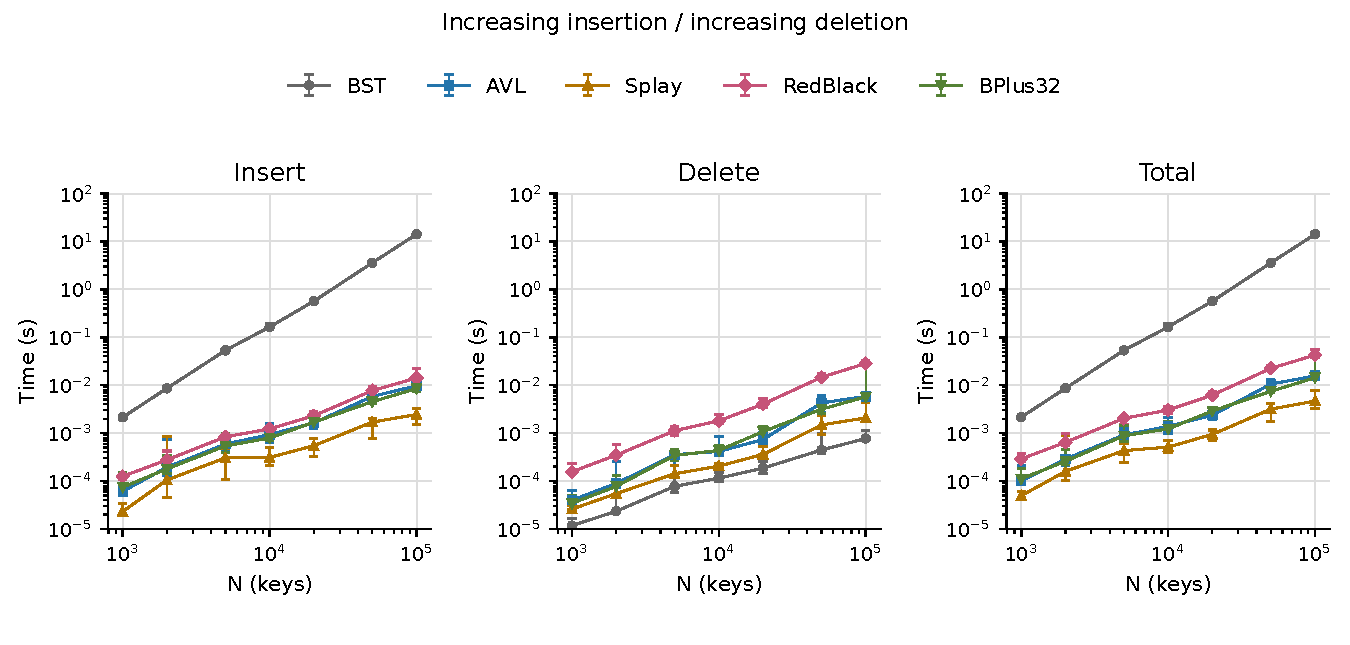
\includegraphics[width=\textwidth]{figures/increasing_same.pdf}
\caption{Increasing insertion / increasing deletion. Each phase uses the same scale as its counterpart in the other scenarios.}
\end{figure}

\begin{figure}[htbp]
\centering
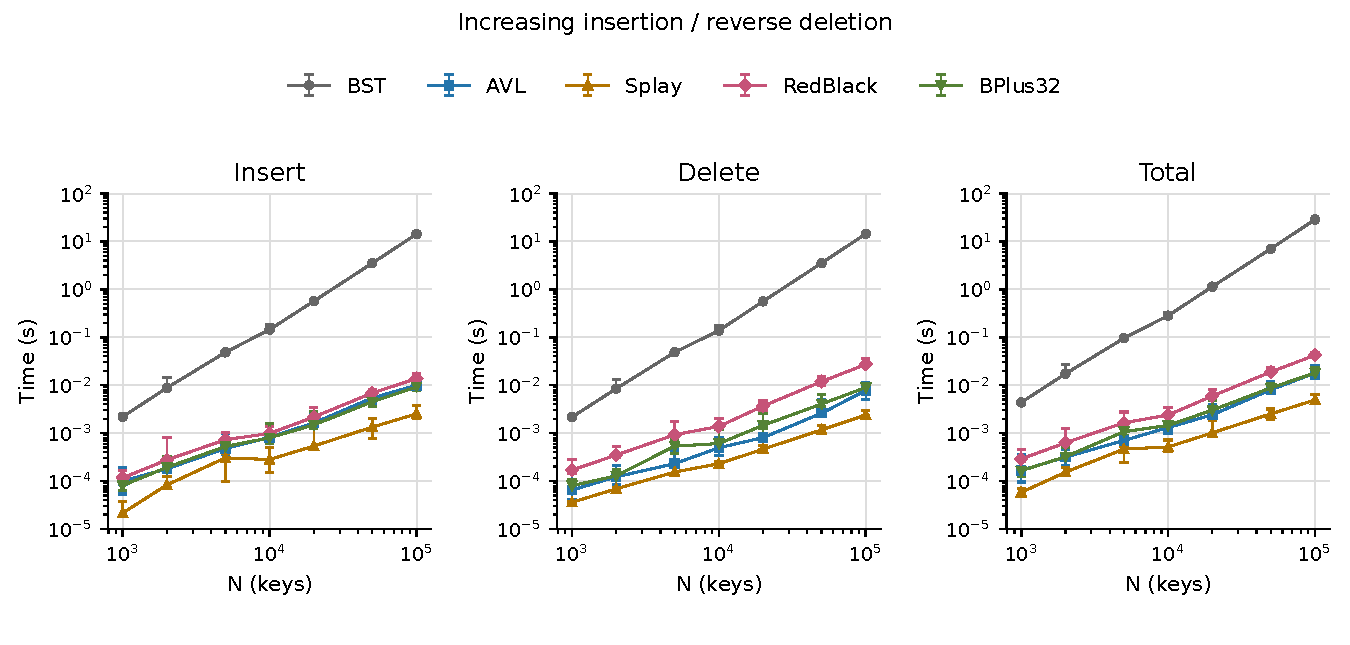
\includegraphics[width=\textwidth]{figures/increasing_reverse.pdf}
\caption{Increasing insertion / reverse deletion. Each phase uses the same scale as its counterpart in the other scenarios.}
\end{figure}

\begin{figure}[htbp]
\centering
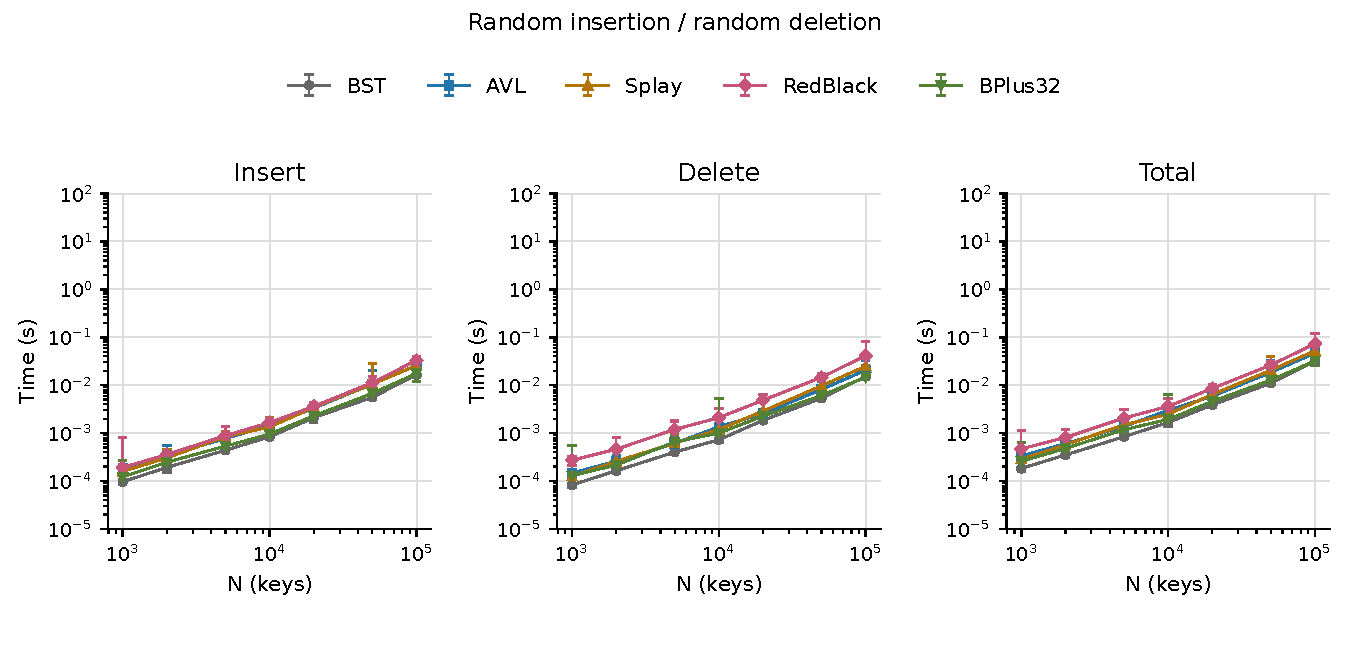
\includegraphics[width=\textwidth]{figures/random_random.pdf}
\caption{Random insertion / random deletion. Each phase uses the same scale as its counterpart in the other scenarios.}
\end{figure}

\section{Analysis and Comments}

\subsection{Time Complexity}

\begin{table}[H]
\centering
\small
\caption{Asymptotic costs for the implemented update operations.}
\begin{tabularx}{\textwidth}{lXX}
\toprule
Tree & Single insertion / deletion & Full sequence of N insertions and N deletions \\
\midrule
BST & O(h); O(N) worst case & O(N\textasciicircum{}2) worst case; expected O(N log N) for random insertion \\
AVL & O(log N) worst case & O(N log N) \\
Splay & O(log N) amortized; O(N) worst case & O(N log N) amortized bound; O(N) for increasing insertion followed by reverse deletion \\
RedBlack (LLRB) & O(log N) worst case & O(N log N) \\
BPlus32 & O(log N), with B = 32 fixed & O(N log N) \\
\bottomrule
\end{tabularx}
\end{table}
\FloatBarrier

\subsubsection{Why Sorted BST Updates Are Quadratic}

Increasing insertion into the plain BST creates a right chain. The ith insertion traverses i-1 existing nodes, so insertion performs N(N-1)/\allowbreak{}2 node visits and takes Theta(N\textasciicircum{}2) time. Increasing deletion repeatedly removes the root and takes Theta(N) total time. Reverse deletion repeatedly searches the longest remaining chain, giving another Theta(N\textasciicircum{}2) phase. Both ordered scenarios have quadratic total cost, but their deletion phases are very different.

The two ordered scenarios share the same insertion phase, and the measured BST insertion time grows by 98.40 and 99.63 times from N=10,000 to N=100,000 across them; the two values differ only through median noise. The ideal quadratic factor is 100, and allocator placement, cache behavior, and scheduling explain why a finite measurement falls short of it.

\subsubsection{Why Splay Benefits from Ordered Updates}

During increasing insertion the largest key is already at the root, so each insertion costs constant work; the result can be a left chain, showing that low total update cost does not require low height at every instant. Reverse deletion removes the current maximum at the root and exposes its left subtree, taking constant work per deletion. Increasing deletion instead splays and removes the current minimum; the first such deletion must traverse the initial left chain and costs Theta(N), so constant time cannot be claimed for each deletion. The general amortized theorem bounds the whole update sequence by O(N log N); the linear insertion and reverse-deletion bounds follow directly from this implementation. \href{https://www.cs.cmu.edu/~sleator/papers/self-adjusting.pdf}{Source: Sleator and Tarjan, Self-Adjusting Binary Search Trees}.

\subsection{Measured Comparison}

At N=100,000, for increasing insertion /\allowbreak{} increasing deletion Splay is fastest (3.402 ms) and BST slowest (10999.209 ms), a 3232.85-fold difference, giving the order Splay, BPlus32, AVL, RedBlack, BST; for increasing insertion /\allowbreak{} reverse deletion Splay is fastest (3.894 ms) and BST slowest (21933.532 ms), a 5633.15-fold difference, giving the order Splay, BPlus32, AVL, RedBlack, BST; for random insertion /\allowbreak{} random deletion BPlus32 is fastest (22.443 ms) and RedBlack slowest (52.854 ms), a 2.35-fold difference, giving the order BPlus32, BST, AVL, Splay, RedBlack. This ordering describes this experiment and does not establish a universal ranking.

The measured ordering follows from how each implementation reacts to the insertion and deletion order:

\begin{enumerate}
  \item BST: no balance rule at all, so insertion order decides everything. Increasing insertion builds a right chain and both ordered scenarios are quadratic, while random insertion avoids that chain and is much cheaper.
  \item AVL: cached heights keep the height logarithmic for every input order, and the strict balance rule makes its cost the least sensitive to order.
  \item Splay: stores no balance information and pays restructuring on random accesses, but adapts to ordered ones, where the key being reached is already at or near the root.
  \item RedBlack: also logarithmic for any order, using color and black-height rules instead of AVL height differences. The deletion routine here performs one extra membership descent. Rotation counts were not measured, so this experiment does not establish that LLRB rotates less than AVL.
  \item BPlus32: a different cost profile rather than a different balance rule. Far fewer levels are visited, but each visit costs a binary search, possible array shifts, and a separator refresh at every modified ancestor.
\end{enumerate}

The comparison therefore measures complete implementations with shared set semantics rather than isolating one balancing primitive.

\subsection{Space Complexity}

All five structures store O(N) total tree memory for fixed B, and they differ in what each node carries and in the auxiliary space of an update:

\begin{enumerate}
  \item BST: two child pointers per node and no balance metadata; updates and destruction run in O(1) auxiliary space.
  \item AVL: the BST layout plus a cached height; recursive updates use O(log N) stack space.
  \item Splay: the BST layout unchanged, with O(1) auxiliary space, since it stores no balance information.
  \item RedBlack: the BST layout plus an int color flag in this implementation; recursive updates use O(log N) stack space.
  \item BPlus32: O(N/\allowbreak{}B) nodes, each reserving O(B) key and child slots, and O(log\_\allowbreak{}B N) recursive stack space. Its leaf layout also reserves child-pointer slots, so reducing the node count does not by itself prove lower byte consumption.
\end{enumerate}

The driver stores two N-key arrays, requiring O(N) input memory, in addition to whatever the tree under test holds. That input memory is separate from update auxiliary memory. The experiment does not measure peak resident memory, so no empirical memory ranking is reported.

\subsection{Limitations and Improvements}

\begin{itemize}
  \item Statistics: only three runs; interpret small differences with observed ranges and use more repetitions.
  \item Workloads: only build-then-delete integer tests; add mixed operations and search benchmarks. Random BST results apply to these shuffled sets.
  \item Instrumentation: comparison and rotation counts were not measured; collect them in a separate instrumented build.
  \item Parameters and environment: vary B+ capacity and pin CPU affinity to assess parameter effects and reduce timing noise.
  \item Page I/\allowbreak{}O: this in-memory benchmark does not measure disk access; use a disk-backed B+ tree to evaluate page I/\allowbreak{}O.
\end{itemize}

\subsection{Conclusion}

Operation order affects tree performance. Sorted insertions turn a plain BST into a chain, giving quadratic total time. AVL and red-black trees maintain logarithmic height through balancing. In this experiment, Splay was fastest for both ordered workloads, while BPlus32 was fastest for the random workload at N = 100,000. These results show that the best choice depends on the workload, within the implementation and measurement limits discussed above.

\section{Author List}

The author and group identifier are recorded on the cover. No division of work among additional contributors is asserted because contributor-specific information was not supplied.


\clearpage
\appendix
\ctexset{section = {number = \Alph{section}}}
\linespread{1}\selectfont\lstset{basicstyle=\ttfamily\fontsize{8}{10}\selectfont,aboveskip=0.4em,belowskip=0.4em}
\section{Source Code Appendix}

The complete implementation is submitted as six C files in src/\allowbreak{}: one per tree, plus src/\allowbreak{}test.c, which includes them and holds the driver, the smoke test, and the benchmark. The excerpts below show the three least obvious repairs, one from each of the trees whose repairs are hardest to follow; the other files also contain insertion, membership, and destruction. Comments explain operation contracts, structural assumptions, and local transformations.

\subsection{AvlBalance}

\lstinputlisting[language=C,firstline=75,lastline=99,caption={avl.c: AvlBalance}]{src/avl.c}

\subsection{MoveRedLeft}

\lstinputlisting[language=C,firstline=126,lastline=140,caption={redblack.c: MoveRedLeft}]{src/redblack.c}

\clearpage
\subsection{RepairChild}

\lstinputlisting[language=C,basicstyle=\ttfamily\fontsize{8}{9}\selectfont,firstline=167,lastline=237,caption={bplus.c: RepairChild}]{src/bplus.c}

\end{document}
